\chapter{Related Works And Theoretical Background}
\label{cha:second_chapter}
This chapter presents the related work that have been done in healthcare and introduces the theoretical background upon which this work is built, with the aim of providing the reader the knowledge he needs to better understand it. 

\section{Related Works}
\label{sec:second_section}

\subsection{Artificial Intelligence in healthcare}
\label{subsec:ai_in_healtcare}
The term~\ac{AI} was coined in 1956 during a workshop in Dartmouth College by John McCarthy, who defined it as <<the science and engineering of making intelligent machines \omissis>> \cite{mccarthy1998artificial}.
One of the first application of~\ac{AI} to healthcare dates back to 1970s, when a team of experts at Stanford University developed the system MYCIN \cite{shortliffe2012computer}. The goal of the project was to create a tool able to identify bacteria causing infections and to recommend antibiotics based on patient's weight. MYCIN used a knowledge base composed by almost 600 rules and an inference engine that applied logical rules to it in order to deduce new information. Despite it was able to achieve results comparable to that of specialists, it was never used in practice, both because it required more computing power and memory than that available in most of the hospital at the time and also because it required a user to enter all relevant information about a patient by typing in responses to some questions that MYCIN posed.

\vspace{5mm} %5mm vertical space
During the 1980s and 1990s several other approaches have been explored in order to enhance the healthcare. Klaus-Peter Adlassnig \cite{fuzzytheory} proposed, in 1980, a model to assist medical diagnosis based on L.A. Zadeh theory of Fuzzy Sets \cite{ZADEH}, well suited for medical applications because it can deal with the inherent ambiguity of medical data. Basilio et al. \cite{Sierra98predictingthe} in 1998 combined Genetic Algorithms \cite{holland:adaptation} and Bayesian Networks \cite{pearl1985bayesian} to predict survival in patient with malignant skin melanoma.

\vspace{5mm}
But among all the different approaches that have been explored, the most used has been, judging by the volume of publications \cite{steimann2001use}, ~\acp{ANN}, introduced for the first time by W.S. McCulloch and W. Pitts in 1943 \cite{mcculloch1943logical}. They are a computing system inspired by animal's biological neural network, able to recognize patterns that are too complex or numerous for a human to extract. Because of their ability to recognise and exploit the intricate relationship among different variables,~\acp{ANN} have been successfully used in many clinical scenarios. 

\noindent One of the first work involving~\ac{ANN} applied to the medical field has been proposed by W.G Baxt in 1990, when he realized a system for the diagnosis of myocardial infarction by means of an~\ac{ANN}. Since then many other application involving Neural Networks has been proposed, for example to identify epilepsy \cite{epilepsy}, appendicitis \cite{appendicitis} and cancer \cite{cancer}.

\noindent During the last fifty years~\ac{AI} has been widely used for healthcare-related applications. Nowadays it's usage is related, but not limited, to disease diagnosis, medical images analysis, prognosis, drug interactions and genomics.


\subsection{Convolutional Neural Networks in computer vision}
\label{subsec:convolutional_neural_networks}
In 1989 LeCun et al. \cite{lecun} introduced one of the first Convolutional Neural Network, a special type of \ac{ANN} particularly effective for the task of analyzing visual images. In their work, specifically, they used it to recognize handwritten zip code numbers. The novelty with respect previous approaches was that the learning process was fully automatic, in the sense that the features used to make the classification were learned by the network instead of being manually designed by a human being. Since their introduction, \acp{CNN} have been widely used for many tasks. The most straightforward is that of image classification, in which an image is given as input to the network and it's assigned to a given class (Figure~\ref{fig:first_figure}).
\begin{figure}[htbp!]
\centering
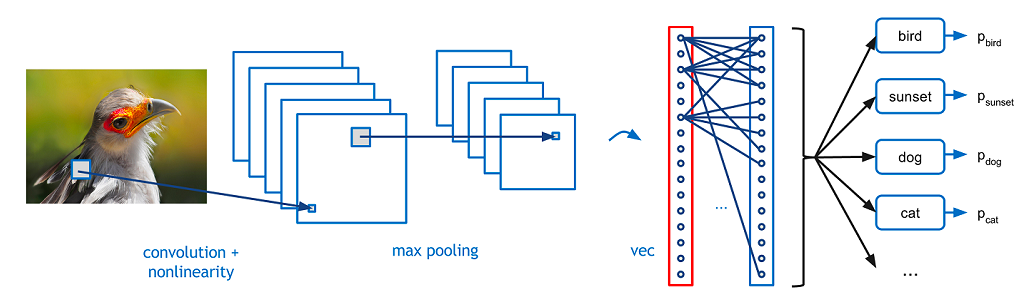
\includegraphics[width=0.95\textwidth]{Tesi/images/image_classification}
\caption{Image Classification using a \ac{CNN}.}
\label{fig:first_figure}
\end{figure}

\newpage

One of the most interesting peculiarity of \acp{CNN} applied to the task of image classification is their ability to explain which part of the picture they are looking at while assigning the class. This can be done by producing a \ac{CAM}, a 2D grid of scores computed for every location of the input image, indicating how important is each location with respect to a given class. Figure~\ref{fig:second_figure} shows an example of \ac{CAM}s produced while assigning the labels "cat" and "dog" to the image given as input. As we can see the network is looking at the correct part of the image, paying attention at the top area to classify the dog and at the bottom one to classify the cat. 

\begin{figure}[htbp!]
\centering
\includegraphics[width=0.85\textwidth,height=0.2\textheight]{Tesi/images/CAM}
\caption{Example of Class Activation Map \cite{cam_paper}.}
\label{fig:second_figure}
\end{figure}


\subsection{Deep Learning in Chest X-Ray Diagnosis}
\label{subsec:convolutional_neural_networks}
During the last years the problem of \ac{CXR} diagnosis has been tackled multiple times using different approaches. One of the major drawbacks of \ac{DL} is that it requires a massive amount of data in order to achieve good results. The first public dataset containing a significant amount of labeled radiography is "ChestX-ray8", that has been release in 2017 by the National Institute of Health \cite{Wang_2017}. It is composed by 108,948 frontal-view X-Ray images coming from 32,717 unique patients. Each radiography is associated with 8 different labels (subsequently increased to 14), each one referring to a particular disease. Among the large amount of work that has been done by the scientific community using this dataset, it worth mentioning that of Rajpurkar et al. \cite{rajpurkar2017chexnet}, able to achieve performance statistically significantly higher than radiologist. In 2019 two new dataset has been released: Chexpert~\cite{irvin2019chexpert}, composed by 224,316 chest radiographs of 65,240 patients, and MIMIC-CXR-JPG~\cite{johnson2019mimiccxrjpg}, made of 377,110 images. \ac{CXR}s from the two dataset are provided with the same 14 labels, that have been extracted from radiology report using \ac{NLP}. 
\newpage
\section{Neural Networks}
\label{sec:Neural Network}
\acp{FCNN} are a computing system able to catch the relationship binding an input to an output. They are based on a Supervised Learning paradigm: in order to learn the function mapping an input to its corresponding output, the network must be trained using a lot of examples composed by both the input and the desired output. 
\vspace{5mm}

A \ac{FCNN} is made of a series of hidden layers, each one composed by a given number of elementary units, called artificial neurons, that are fully connected to the ones belonging to the previous layer. When the network receives an input, it pass through all the network and gets transformed by the artificial neurons, until it reaches the last layer, where an output is carried out (Figure \ref{fig:third_figure}).
\begin{figure}[htbp!]
\centering
\includegraphics[scale=0.45]{Tesi/images/FCNN}
\caption{Fully Connected Neural Network}
\label{fig:third_figure}
\end{figure}

\vspace{5mm}
This model, however, is not suitable for image processing. Indeed, if we consider, for example, an image with shape $32 \times 32 \times 3$ pixels, a single neuron in the first hidden layer of a \ac{FCNN} would have a number of connections equal to 32*32*3 = 3072. Although it seems to be a reasonable amount of weights, this approach does not scale well when we are dealing with larger images. As we will see in next chapters, our images will have a size of $224 \times 224 \times 3$, using \ac{FCNN} would lead a single neuron to have 150,528 connections. Such a number of parameter is intractable and would lead to overfitting.

\subsection{Convolutional Neural Network}
\label{sec:convolutional_neural_network}
Convolutional Neural Networks are a particular type of Neural Networks that have been extensively used over the past years, able to overcome the limits of \ac{FCNN} discussed in section \ref{sec:Neural Network}. \acp{CNN} have been successfully used for the first time by Yann Lecun for the task of recognizing handwritten digits \cite{lecun}.
The most important building block introduced with \acp{CNN} is the convolutional layer, designed to take advantage of the multi-dimensional structure of the input. Neurons in the first convolutional layer are not connected to every single pixel of the input image, but only to a small part of it, the so called receptive field. \acp{CNN} have a hierarchical structure: in the first layers the network extracts simple patterns, such as edges and curves that, in the following layers, are assembled to generate higher level features (Figure \ref{fig:fourth_figure}).
\begin{figure}[htbp!]
\centering
\includegraphics[width=0.90\textwidth]{Tesi/images/Feature}
\caption{Feature hierarchy in a \ac{CNN}}
\label{fig:fourth_figure}
\end{figure}

Feature extraction is accomplished by the so called kernels (also known as filter). Figure \ref{fig:fifth_figure} shows an example of two kernels applied to an image: in the top left picture a vertical filter has been used, thus all the vertical lines in the original image gets enhanced, while the rest gets blurred. The top-right image, instead, shows what happen when an horizontal filter is applied. Of course kernels do not have to be defined manually, during the training phase the convolutional layers will automatically learn the most useful for the given task and the subsequent layers will learn to combine them into more complex pattern.
\vspace{5mm}
\begin{figure}[htbp!]
\centering
\includegraphics[scale=0.8]{Tesi/images/FeatureMap}
\caption{Example of filters applied to an image \cite{mlbook}}
\label{fig:fifth_figure}
\end{figure}

\vspace{5mm} %5mm vertical space

The mathematical operation that allows the network to extract the features from the input image is called convolution, that consist in sliding a kernel (that is basically a small matrix of number), across the whole dimensions of the input and compute the dot product between the entries of the filter and the input at any position. Convolution between image $I$ and kernel $w$ of size $k \times k$ can be computed as:
\begin{equation} \label{eq:first_equation}
\begin{gathered}
(I\ast w)\left [ r,c \right ]  = \sum_{x=-k}^{k}  \sum_{y=-k}^{k} w(x,y)I(r-x, c-y)
\end{gathered}
\end{equation}

\noindent An example of convolution is shown in Figure \ref{fig:sixth_figure}, in which the value of the destination pixel has been computed as: 
\begin{equation} \label{eq:second_equation}
\begin{gathered}
(4 \cdot  0) + (0 \cdot  0) + (0 \cdot  0) + (0 \cdot  0) + (0 \cdot  1) + (0 \cdot  1) + (0 \cdot  0) + (0 \cdot  1) + (-4 \cdot  2) = -8
\end{gathered}
\end{equation}

\begin{figure}[htbp!]
\centering
\includegraphics[scale=0.7]{Tesi/images/convolution}
\caption{Example of convolution operation between an image and a kernel}
\label{fig:sixth_figure}
\end{figure}

\newpage

\vspace{5mm} %5mm vertical space
\noindent Another widely used layer in \acp{CNN} is the Pooling Layer. Its function is to progressively decrease the spatial size of the representation in order to reduce the computational load, the memory usage and the number of parameter (preventing thereby the risk of overfitting). A pooling layer has no weights, what it does is to aggregate the input using an aggregation function, such as mean or max (Figure \ref{fig:seventh_figure}). A max pooling layer, moreover, introduces some level of invariance to small translations, a feature that could be useful for the task of image classification.


\begin{figure}[htbp!]
\centering
\includegraphics[width=0.95\textwidth]{Tesi/images/pooling}
\caption{Example of Max Pooling}
\label{fig:seventh_figure}
\end{figure}

\subsection{Class Activation Map}
\label{sec:cam}
In 2016 Zhou et al. \cite{zhou2015cnnlocalization} shown that a \ac{CNN} is able to identify exactly which region of an image is used for discrimination. The novelty with respect to previous works is that the network is only trained for solving the  classification task, thus no bounding box annotation is provided as input to the network. 
The remarkable localization ability of \ac{CNN} is lost when the fully connected layer is used for classification. Thanks to the work of Lin et al. \cite{gap}, this problem can be overcome by means of a \ac{GAP} layer, initially introduced to minimize the number of parameters, avoiding the usage of fully connected layer while maintaining high classification performance. 
Similarly to Pooling Layers, a \ac{GAP} layer aims at reducing the spatial dimension of the input tensor. However \ac{GAP} makes a more extreme type of dimensionality reduction, transforming a three dimensional input of size $h \times w \times d$ into a tensor with shape $1 \times 1 \times d$ (Figure \ref{fig:eigth_figure}).

\begin{figure}[htbp!]
\centering
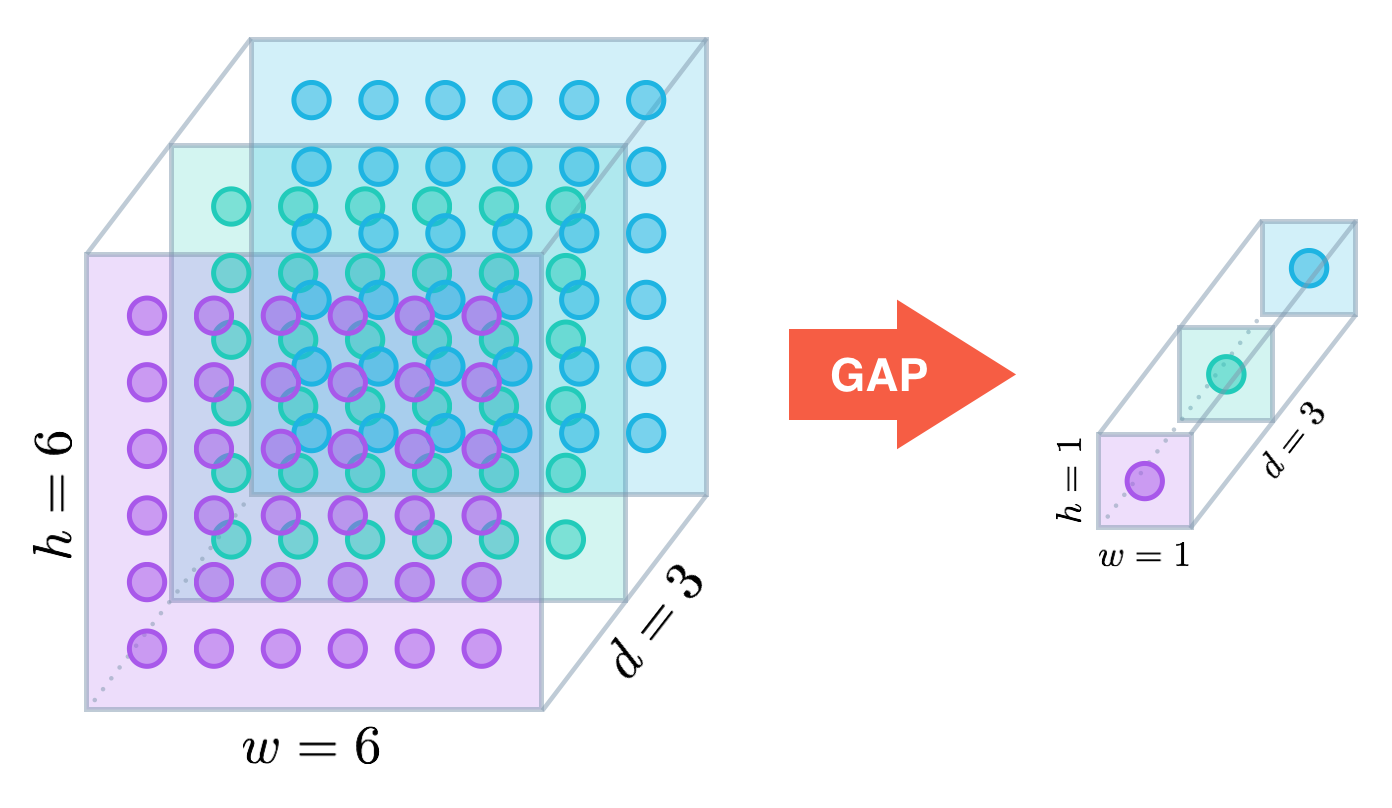
\includegraphics[scale=0.5]{Tesi/images/GAP}
\caption{Example of Globale Average Pooling \cite{gap_image}.}
\label{fig:eigth_figure}
\end{figure}

\noindent In order to generate the \ac{CAM}, we will make a weighted sum of the feature maps at the last convolutional layer. If we indicate with $f_{k}(x,y)$ the activation of unit k at spatial location $(x,y)$ then the result of performing Global Average Pooling is given by:

  \begin{equation}
  \label{eq:third_equation}
  \begin{gathered}
  F_{k} = \sum_{x,y} f_{k}(x,y)
  \end{gathered}  
  \end{equation}
  
\vspace{3mm}

\noindent Thus the input to the softmax for a given class will be:
 \begin{equation}
  \label{eq:fourth_equation}
  \begin{gathered}
  S_{c} = \sum_{k} w_{k}^{c} F_{k} = \sum_{x,y} \sum_{k} w_{k}^{c} f_{k}(x,y)
  \end{gathered}  
  \end{equation}
  
\vspace{3mm}

\noindent Essentially $w_{k}^{c}$ represent the importance of $F_{k}$ for class $c$. Once $S_{c}$ has been calculated, the probability for a class $c$ can be computed using the softmax function: 
\begin{equation}
\label{eq:fifth_equation}
\begin{gathered}
P_{c} = \frac{exp(S_{c})}{\sum_{c} exp(S_{c})}
\end{gathered}  
\end{equation}
\vspace{3mm}

\noindent While the Class Activation Map for class $c$, instead, can be computed as : 

  \begin{equation}
\label{eq:sixth_equation}
\begin{gathered}
M_{c}(x,y) = \sum _{k} w_{k}^{c} f_{k}(x,y)
\end{gathered}  
\end{equation}
  
\noindent So in order to extract the most important part of the image for a given class, we project back the weights of the output layer on the convolutional feature maps obtained from the last Convolution Layer. Image \ref{fig:ninth_figure}, taken from the work of Zhou et al. \cite{cam_paper}, shows how the \ac{CAM} is computed by making a weighted sum of the last convolutional layer's features.

\begin{figure}[htbp!]
\centering
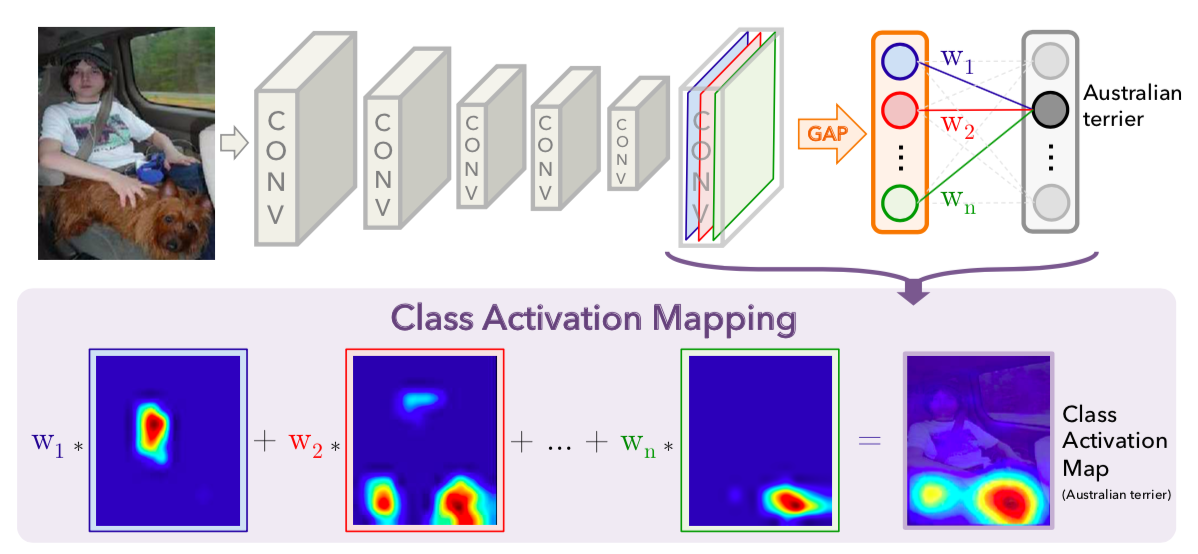
\includegraphics[scale=0.35]{Tesi/images/Class Activation Map}
\caption{Class Activation Map generation.}
\label{fig:ninth_figure}
\end{figure}

\subsection{Embedding}
\label{sec:embedding}
In the context of \ac{ANN} a very useful techniques is Embedding. When dealing with images, we generally work with a massive amount of data. A simple colored image with resolution of $224 \times 224$ pixels is converted into a tensor having $224 \times 224 \times 3 = 150.528$ entries. Although \acp{CNN} are able to deal with such a large amount of data, the vast majority of algorithms can't process it in a reasonable amount of time.
In order to overcome this issue we can rely on Embedding, a set of techniques used to reduce the input dimension. An embedding is a learned low dimensional vector representing the input. Once an embedding has been extracted, it somehow contains the same relevant information of the input but in a smaller and more manageable representation, suitable for being used by other kind of algorithms. 

\vspace{5mm}

\acp{CNN} can be used to extract the low dimensional feature vector. In the hidden layers, in fact, the network learns a representation of the input that is subsequently used for classification. If we cut the network at one of the hidden layer, thus, we can extract a low dimension vector representing the the input (Figure \ref{fig:tenth_figure}).


\begin{figure}[htbp!]
\centering
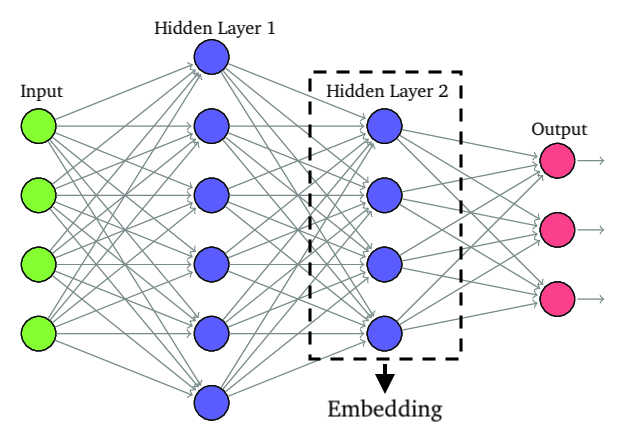
\includegraphics[scale=0.5]{Tesi/images/Embedding}
\caption{Embedding extraction from an \ac{ANN}}
\label{fig:tenth_figure}
\end{figure}


\section{Ensemble Learning}
\label{sec:ensemble}
In social science there is a theory, called "The Wisdom of Crowd", stating that the aggregate decision made by a group of people will often be better than those of it's individual members \cite{crowd}. A similar idea is exploited by Ensemble Learning, a technique that allows to improve machine learning results by combining several models. Figure \ref{fig:eleventh_figure} shows a typical workflow exploiting ensemble: several classifiers are trained and then combined in order to carry out a single prediction that takes care of the opinion coming from all the base classifiers. 
\begin{figure}[htbp!]
\centering
\includegraphics[scale=0.35]{Tesi/images/Ensemble.pdf}
\caption{Ensemble Learning}
\label{fig:eleventh_figure}
\end{figure}
The keypoint here is to find the best way to combine all the predictions. There are  different approaches, such as:
\begin{itemize}
  \item \textbf{Ensemble Averaging}: the predictions that are carried out from the single experts are merged together using either a mere average or a weighted sum. Doing this helps reducing the variance of the output.
  For example, if we indicate as $y_{i}$ the output of each base classifier, then the ensemble of the $n$ experts can be computed as:
  \begin{equation}
  \label{eq:seventh_equation}
  \begin{gathered}
  \bar{y}(\mathbf{x},\alpha) = \sum_{i=1}^{n} \alpha_i y_{i}(\mathbf{x})
  \end{gathered}  
  \end{equation}
  \item \textbf{Bootstrap Aggregating}: also known as Bagging \cite{bagging}, this technique aims at reducing the variance by averaging the output of multiple models built on different training set. More specifically, given a dataset $D$, each model if fitted using a dataset $D_{i}$ build by sampling uniformly and with replacement from $D$.
  
  \item \textbf{Boosting}: this aggregation approach aims at producing a strong predictor by incrementally building the weak classifiers. It's peculiarity is that each model instance is trained paying more attention to the samples that were misclassified by the previous predictor.
  
  
  \item \textbf{Stacking}: this approach combines multiple classification or regression models using a meta-classifier or a meta-regressor. Specifically, a training set is used to train the base classifiers, then the predictions that are carried from the classifiers are used as feature to train the meta-learner. The pseudocode for the general stacking algorithm is shown in figure \ref{fig:twelfth_figure}
  \begin{figure}[htbp!]
\centering
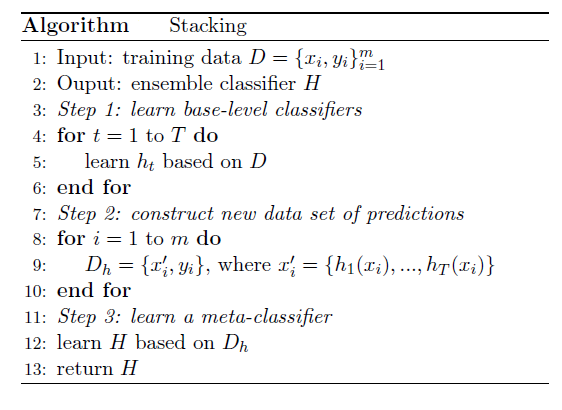
\includegraphics[scale=0.55]{Tesi/images/stacking_pseudocode.png}
\caption{Stacking Pseudocode}
\label{fig:twelfth_figure}
\end{figure}
  
    \end{itemize}


\section{Random Forest}
\label{sec:random_forest}
Random Forests are an ensemble algorithm proposed by T.K. Ho in 1995 \cite{random_forest}. The idea behind \acp{RF} is to build a multitude of decision trees and combine their predictions.

\noindent Decision Trees are a supervised-learning method used bot for classification and regression tasks. The algorithm builds a tree-like structure in which:
\begin{itemize}
    \item An internal node is a test on an attribute.
    \item A branch represent an outcome of the test.
    \item A leaf represent a class label or a class label distribution.
\end{itemize}


\noindent Figure \ref{fig:thirteenth_figure} shows an example of Decision Tree used to predict survivals on Titanic. A new instance is assigned to a class by following a path starting from the root and ending in a leaf node, testing a different feature at each internal node.

\begin{figure}[htbp!]
\centering
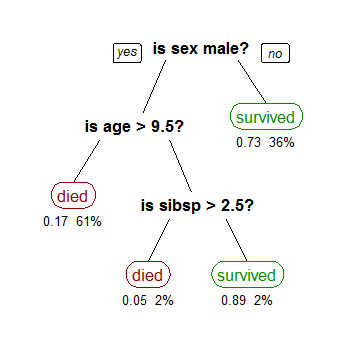
\includegraphics[scale=0.7]{Tesi/images/CART_tree_titanic_survivors.png}
\caption{Decision Tree showing survival of passenger on Titanic \cite{pict}}
\label{fig:thirteenth_figure}
\end{figure}
  
Decision Trees have many advantages: they are very fast in making predictions and, differently from \acp{ANN}, they are a white box model, in the sense that they are easy to interpret and visualize. Indeed it's possible to easily check which are the features that most contribute to carry out a particular prediction. However, they also have some drawback. They often create over-complex structure that are not able to generalize well, thus leading to overfitting. Another big issue is that they are unstable, in the sense that a small variation in the training data may generate a totally different model.
These issues can be overcome by resorting to Random Forest, that are basically an ensemble of Decision Trees based on Bagging, a technique seen in section \ref{sec:ensemble}.
The main steps to build a Random Forest are the following:
\begin{itemize}
    \item Build $k$ training set $D_{i}$ by sampling with replacement from $D$
    \item Learn tree $T_{i}$ from $D_{i}$ using only a random subset of the input variables.
    \item Save the tree as it is, without performing any pruning
\end{itemize}
Once the Random Forest has been created, the predictions computed by the trees are combined using:
\begin{itemize}
    \item Majority Voting (in the case of Classification)
    \item Average (in the case of Regression)
\end{itemize}

When the number of trees is sufficiently large, Random Forest can prevent overfitting. Moreover they are an easy to use tool, having only two important parameters to tune (number of trees and percentage of variables for split).
  \begin{figure}[htbp!]
\centering
\includegraphics[scale=0.35]{Tesi/images/rf.pdf}
\caption{Example of Random Forest for classification task}
\label{fig:fourteenth_figure}
\end{figure}


\section{Gradient Boosting}
\label{sec:gradient_boosting}
Gradient Boosting is a learning algorithm proposed in 1990 by Friedman \cite{gradient_boosting}. As the name suggests, it's a technique based on boosting. The idea of this algorithm can be summarized by the following steps:
\begin{enumerate}
    \item Learn a predictor.
    \item Compute the error residual.
    \item Learn to predict the residual
    \item Goto point 2
\end{enumerate}

\noindent So Gradient Boosting tries to repetitively leverage the patterns in the residuals to improve the successive predictions.
The predictors used as weak leaerner in gradient boosting are decision trees. Note that, however, gradient boosting is a greedy algorithm and, thus, it can overfit the dataset quickly. A solution to this problem is that of constraining the trees, being the shallow trees, generally, less prone to overfitting.


\section{Summary}
\label{sec:sec_chapter_sumary}
The goal of this chapter was to give an general overview of the main techniques that will be used in the following chapters. We've seen what Artificial Neural Networks are and how they can be used in order to deal with images, both for classify them and localize interesting areas. We've also seen how multiple approaches can be combined together to enhance the global performance, with a particular attention on Random Forest. In the next chapter we will introduce the dataset and we'll describe the pre-processing phase.